 \documentclass[oneside,11pt]{article}


\usepackage{soul}
\usepackage{natbib}
\usepackage{hyperref}
\usepackage{bookmark}
\usepackage{graphicx}             
\graphicspath{{./Figuras/}}
\usepackage[dvipsnames]{xcolor}
\usepackage{todonotes}
\usepackage{makecell}
\usepackage[margin=1in]{geometry}
\usepackage{float}                
\usepackage{amsmath}
\usepackage{amscd}
\usepackage{amsfonts}
\usepackage{amssymb}
\usepackage{bbm}
\usepackage{booktabs}
\usepackage{nameref}
\usepackage{multirow}
\usepackage[nokeyprefix]{refstyle}
\usepackage{rotating}
\usepackage{threeparttable}
\usepackage{afterpage}
\usepackage{lscape}
\usepackage{enumerate}
\usepackage{caption}
\usepackage{subcaption}
\usepackage{epstopdf}
\usepackage{setspace}
\usepackage{svg}
\usepackage{dsfont}
\usepackage{amsthm}
\usepackage{tocloft}
\usepackage{etoc}
\usepackage{lmodern}
\usepackage{bm}
\usepackage[T1]{fontenc}
\usepackage{tgpagella}

\epstopdfDeclareGraphicsRule{.tiff}{png}{.png}{convert #1 \OutputFile}
\AppendGraphicsExtensions{.tiff}

\epstopdfDeclareGraphicsRule{.tif}{png}{.png}{convert #1 \OutputFile}
\AppendGraphicsExtensions{.tif}

\def\sym#1{\ifmmode^{#1}\else\(^{#1}\)\fi}

\usepackage{tikz}
\usetikzlibrary{shapes.geometric, arrows}
\usetikzlibrary{calc}
\usetikzlibrary{matrix}

\tikzset{ 
    table/.style={
        matrix of nodes,
        row sep=-\pgflinewidth,
        column sep=-\pgflinewidth,
        nodes={
            rectangle,
            draw=black,
            align=center
        },
        minimum height=1.5em,
        text depth=0.5ex,
        text height=2ex,
        nodes in empty cells,
%%
        every even row/.style={
            nodes={fill=gray!20}
        },
        column 1/.style={
            nodes={text width=2em,font=\bfseries}
        },
        row 1/.style={
            nodes={
                fill=black,
                text=white,
                font=\bfseries
            }
        }
    }
}


\usepackage{colortbl}
\usepackage{url}
\urlstyle{rm}
\definecolor{darkblue}{rgb}{0,0,.4}
\hypersetup{colorlinks=true, breaklinks=true, citecolor=Maroon, linkcolor=darkblue, menucolor=darkblue, urlcolor=darkblue}

\newtheorem{theorem}{Theorem}
\newtheorem{claim}[theorem]{Claim}
\newtheorem{prop}[theorem]{Proposition} 
\newtheorem{cor}[theorem]{Corollary} 
\newtheorem{assumption}{Assumption} 
\newtheorem{lem}{Lemma} 

\DeclareRobustCommand{\hlgr}[1]{{\sethlcolor{green}\hl{#1}}}


\usepackage{comment}
%para esconder columnas en tablas (enrique)
\usepackage{array}
\newcolumntype{H}{>{\setbox0=\hbox\bgroup}c<{\egroup}@{}}
\linespread{1.25}

\newcommand{\wh}{\widehat}
\usepackage{anyfontsize}

\usepackage[linesnumbered,vlined,ruled,commentsnumbered]{algorithm2e}

\DontPrintSemicolon
\newcommand{\To}{\mbox{\upshape\bfseries to}}
\newcommand{\E}{\mathbb{E}}

\DeclareCaptionFormat{cont}{#1 (cont.)#2#3\par}
%%% HELPER CODE FOR DEALING WITH EXTERNAL REFERENCES
\usepackage{xr}
\makeatletter
\newcommand*{\addFileDependency}[1]{
  \typeout{(#1)}
  \@addtofilelist{#1}
  \IfFileExists{#1}{}{\typeout{No file #1.}}
}
\makeatother


\newcommand*{\myexternaldocument}[1]{
    \externaldocument{#1}
    \addFileDependency{#1.tex}
    \addFileDependency{#1.aux}
}

%\myexternaldocument{OA}

%%%%%%%%%%%%%%%%%%%%%%%%%%%%%%%% DOCUMENT
\begin{document}

\title{Wage Transparency Induces Wage Increases \thanks{We want to thank.}}
\author{Marco Medina \and Eduardo Alcaraz \and Gabriela López \and Luis Martínez \and Enrique Seira\thanks{Seira: MSU, seiraenr@msu.edu (corresponding author); Alcaraz: IMSS, eduardo.alcarazp@imss.gob.mx; López: IMSS, ; Martínez: IMSS, luis.martinezch@imss.gob.mx; Medina:  ITAM, marco.medina@itam.mx}}
\date{This draft:  \today \\[2 cm]}  %\and Christopher Woodruff


%\vspace{.5in}


\maketitle
\thispagestyle{empty}
\begin{abstract}

Payroll tax evasion can occur by firms underreporting wages. We study whether providing information about enrollment and wages to workers increased wages and whether it causes workers to exit the formal sector. 
We take advantage of the staggered adoption of Mexico's Social Security (IMSS)-created app (\textit{Reporte Personalizado de Cotización en el IMSS (RPCI)}) providing workers with information on their employer-reported wages and status. We find that compared to a control group that has not installed RPCI, wages increased by 5\% of the mean, a substantial amount. We find no effect on workers exiting the formal sector as a result of RPCI. The results suggest that a substantial fraction of workers did not know that their employers were reporting lower wages to IMSS.

\end{abstract}

\vspace{.3in}

\textbf{Keywords:} Informality, wage transparency, tax evasion, Social Security App, RPCI

%\textbf{JEL codes:}

\newpage

\pagenumbering{arabic}
\etocdepthtag.toc{mtchapter}
\etocsettagdepth{mtchapter}{subsection}
\etocsettagdepth{mtappendix}{none}

\section{Introduction} \label{introduction}

According to the International Labour Organization, close to 60 percent of workers worldwide work in the informal sector \citep{ILO_2018}. The informal sector comprises close to a third of economic activity in developing countries, twice as much as in developed ones.\footnote{\url{https://www.imf.org/external/pubs/ft/fandd/2020/12/pdf/what-is-the-informal-economy-basics.pdf}} The prevalence of informality may not be innocuous. Informality facilitates tax evasion, weakening state capacity. Moreover, having some workers and not others be subject to taxes could cause distortions in the allocation of resources, lowering a country's income \citep{Misallocation}. 

A desire to evade payroll taxes occurs along several margins. First, firms themselves may not register with the tax authorities. Second, even if the firm is registered, it may hire workers and not report them to the social security administration (IMSS, for its acronym in Mexico).%, this avoids paying a 24\% payroll tax. 
These two margins are the focus of the important work of \cite{Ulyssea}. A third understudied margin revolves around what wage to declare to tax authorities when both the firm and the worker are registered with tax authorities. Income and payroll taxes create incentives for both firms and workers to report lower salaries. In Mexico, the payroll tax is 24\% of the reported wage, and part of this tax falls de jure on the employer. The employer is mandated to report, collect, and pay the tax to IMSS. This could be beneficial. The literature has found that third-party reporting could help reduce evasion \citep{Denmark}, although, in contexts of low monitoring, it may be less effective: the gains from the worker and employer colluding to report a lower wage are relatively large. \cite{kumler2020enlisting} note that ``having firms report employees’ wages is no guarantee of accurate reporting in a low-enforcement context like Mexico.'' %Being registered with IMSS is mandated by law. 

On the other hand, having the firm and not the worker not be involved in the process of enrolling and reporting wage to IMSS, could lead to unilateral underreporting on the part of firms. We know of anecdotal evidence of workers finding out that they are not registered with IMSS or registered with a small salary without their knowledge. Reporting a low wage has costs for workers that are not incurred by the firm. Being registered with IMSS gives workers access to free medical services regardless of the level of the wage reported. But the amount of disability insurance and the amount contributed to the worker's personal retirement savings account does in fact depend on the reported wage. \cite{kumler2020enlisting} estimate that the median under-reporting of wages in Mexico is close to 30\% for small firms and 56\% for large ones. Could it be that part of this underreporting occurs without the knowledge and consent of workers? 

\cite{kumler2020enlisting} find that a regulatory change that (a) tied the wage reported more closely and positively with retirement savings, and (b) increased wage transparency to the worker, increased wages reported to IMSS, especially for the younger cohorts which were more likely affected by the regulatory change. %Unfortunately, because the reform involved both changes in the benefits and changes in the information provided to workers about the wage reported by their employer, it is not possible to attribute causality among these two. 
It is difficult to know however what aspect of the reform ---wage transparency or incentives to report wages--- is driving the result.\footnote{It is also possible that because the treatment-control comparisons involve comparing older versus younger workers, the differences in differences results could be driven by differential time trends. The reform was implemented just after the tequila crisis, a time of macroeconomic upheaval.} %One the one hand workers can be misinformed and erroneously assume that they are formally registered when in fact they are not. On the other hand, given that workers could collude with the employer on what wage to report, incur fewer taxes, and split the tax savings. \
\cite{kumler2020enlisting} write that the  ``extent workers are aware of underreporting by their employers and, relatedly, to what extent the effects of the pension reform we observe are due to the change in incentives versus the change in information'' are two open questions.  In a large survey to close to more than 100,000 workers that are (were) registered with IMSS, and we directly ask them if they think their current (last) employer registered them in IMSS and whether the entire salary was reported. Almost one-quarter of them say they don't know if their employer reports the entire wage to IMSS, while only 10\% say the employer definitely does not.\footnote{The remaining $67\%$ think their employer reports the complete wage to IMSS.} Interestingly almost 1 in 5 say they explicitly discussed with their employer which wage to report to IMSS. Taken literally, this suggests that part of the misreporting is collusive and workers are likely informed about it, but maybe not a large part. 

The source of underreporting clearly matters as it leads to different policies. If underreporting occurs with the consent of workers, then a policy of government monitoring, audits, and enforcement would be called for. A policy of providing workers with information about their formal status and wage reported should have no effect. But if underreporting occurs behind the worker's back, then we would expect that informing workers about their formality status would lead to changes in behavior, potentially increasing reported wages. It could also lead to worker-employer conflict and lead to employers firing workers with maybe workers suing employers.  

In this paper we test whether giving information to workers about whether their employer has registered them with IMSS, the wage that is registered, and the days reported. To do this we take advantage of an IMSS-created app (\textit{Reporte Personalizado de Cotización del IMSS (RPCI)}) which provides  pieces of information to any Mexican that downloads it. We exploit the staggered adoption of the app which from February 2021 to August 2022 incorporated more than 800,000 new users. The \textit{RPCI} App gives workers a low-cost way to check their formal status in the extensive (begin registered) and intensive margin (how many days of work were registered and at which wage level). Before RPCI workers had to ask for an appointment to an IMSS office, show IDs, and wait your turn to get the information. This could take weeks of delay and hours of waiting in line. In interviews with IMSS officials they estimate that less than \hl{XX\%, EDUARDO} of workers did it.\footnote{\url{https://www.youtube.com/watch?v=phKa31-QH4M}.}

Using IMSS administrative data and the differences-in-differences methodology of \cite{deChaisemartin2022}, we estimate the effect of downloading the RPCI app study on 2 outcomes: reported wages for those that were already registered (intensive margin), and whether workers are more or less likely to keep that job (extensive margin). Effectively we compare early adopters to late adopters and non-adopters, allowing for dynamic and heterogeneous treatment effects. We find that, before adoption, early, late RPCI and non-adopters had similar time trends of wages and employment status (IMSS registration). However, we find wages start to increase exactly when the RPCI App is downloaded, reaching an average increase of 20 pesos 1 year after (close to 5\% of mean wages). This is consistent with an important fraction of workers \textit{not knowing} that their wages were underreported by their employer. We find that the effect is larger for males, older workers (55 to 65), and for those earning 1 to 3 minimum wages, firms that registered agriculture and construction as their industry, and small firms (<50 workers).

Second, one may worry that the information causes conflict between workers and their employers which leads to job loss. Contrary to this, we detect no effect on the likelihood of being registered at IMSS.  %\hl{and we detect no effect of switching to another formal job (MARCO: podemos revisitar este ultimo?}. 
The evidence suggests that a fraction of workers did not know their wages were underreported, and that the RPCI app lead to increased reported wages without leading to job loss. 

The paper proceeds as follows. Section \ref{context} describes the Mexican context and the RPCI app. Section \ref{data} describes our data and the adoption of the app among the population. Section \ref{specification} lays out our methodology, while Section \ref{results} describes our empirical specification and results. Finally Section \ref{conclusion} concludes and suggests ways in which the analysis could be made more comprehensive and more robust.


\section{Context} \label{context}

\vspace{.2in}
\hl{EDUARDO, PUEDES METERLE MANO A EL CONTEXTO SI ES INCORRECTO?}

\subsection{Social security taxes and benefits}

The Mexican social security  or IMSS by its acronym in Spanish is a government institution in Mexico that provides social security services to Mexican citizens and legal residents. IMSS operates as the country's largest healthcare institution and offers a range of services, including healthcare, retirement, disability, and maternity benefits. IMSS plays a vital role in providing healthcare and social security coverage to millions of Mexicans through a network of hospitals, clinics, and medical facilities throughout Mexico. But to access those benefits workers have to be registered with IMSS and subject to a payroll tax at the rate of approximately 24\% of the salary. 

The IMSS system is funded through payroll contributions (taxes) from workers, employers, and the federal government. Payroll Contributions: A portion of employees' salaries is deducted to fund IMSS. The contribution rate is based on a percentage of the employee's salary, and it varies depending on the individual's income level.\footnote{The employee's contribution rate is based on a progressive scale that takes into account their income level. The rates range from 0.625\% to 6.25\% of the employee's base salary, depending on their income bracket.} The contributions are collected by employers and then transferred to IMSS. Employer Contributions: Employers are also required to contribute to IMSS on behalf of their employees at a rate of 20\%. The employer's contribution is separate from the employee's payroll deduction. Government Subsidies: The Mexican government provides subsidies to IMSS to support its operations and ensure the provision of healthcare services to the population.\footnote{According to the Social Security Law, individuals can be affiliated with the IMSS under either the mandatory or voluntary scheme, each with its own set of benefits, eligibility criteria, and financing methods. In our sample 97\% of workers who are affiliated through their employers under the Mandatory Scheme.}

According to the Social Security Law, the benefit scheme of the Mandatory Scheme comprises all the insurance coverage offered by the IMSS: Work-related Risks, Sickness and Maternity, Disability and Life, Retirement, Old Age, and Elderly Unemployment, Daycare Centers, and Social Benefits.
With the exception of Daycare Centers and Social Benefits, the other items' benefits increase as a function of the reported wage.\footnote{The Work-related Risks Insurance offers a temporary disability subsidy equivalent to 100\% of the wage registered at IMSS at the beginning of the disability for a period of up to 52 weeks. Maternity coverage provides a subsidy equivalent to 100\% of the last reported wage for a period of 42 days before and after childbirth. Sickness insurance provides a subsidy equivalent to 60\% of the registered wage for up to 52 weeks. Lastly, the Retirement Benefits are based on the worker's contributions to the social security system throughout their working life. The pension amount is determined by factors such as the worker's average salary, the number of years of contributions, and the retirement age.}  


\subsection{The RPCI initiative}

Importantly, employers report to the IMSS the worker's job status (whether he/she is employed), the wage earned, and the number of days worked in the month. They can do this without the explicit participation of the worker. This means that employers may underreport the actual wage earned by the worker without the worker knowing. Underreporting wages can be detrimental to the worker, since disability insurance and retirement pension benefits depend proportionately on the reported wage. Anecdotally our contacts at IMSS tell of many instances when Workers discover wage underreporting when they ask for their weeks-worked report before retirement and are surprised to find out they have been accumulating lower savings than expected as a result of wage underreporting.  Unfortunately, by the time workers discover underreporting, there is little they can do to rectify the situation. 

To address this issue, the IMSS has implemented the RPCI (\textit{Reporte Personalizado de Cotizaciones en el IMSS}) initiative. The \textit{RPCI} provides workers with easy access to information about their job registration, including their current reported wage and the legal name of their employer. Workers can register for the \textit{RPCI} through the IMSS app and receive their personalized report on a monthly basis after registration. Figure \ref{rpci_example} illustrates a screenshot of the IMSS app and provides an example of the PDF report that workers receive through the RPCI. The objective of this initiative is to enhance workers' access to information regarding their job registration and to promote compliance through worker enforcement.\footnote{Figure \ref{rpci_flyers} shows flyers announcing the RPCI app. Figure \ref{rpci_register} shows how the workers register for the RPCI within the IMSS app.}



%%%%%%%%%%%%%%%%%
%With this in mind, IMSS created the RPCI, a personalized report on the worker's current job, which includes information on the worker's current reported wage and employer's legal name.\footnote{Figure \ref{rpci_example} shows a screenshot of the IMSS app and an example of the RPCI's PDF workers receive.} The objective is to make access to information on the worker's register easier, and increase compliance via enforcement from the workers.

%We conducted an online survey of workers enrolled at IMSS during August 2021. The survey was sent via email to a random sample of workers. Figure \ref{fig:hist_knowledge_register_survey} shows the answers to some of the survey questions, related to knowledge about IMSS and wage reporting to the IMSS. This survey and our findings serve as motivation for this paper.

%We find that not all workers know the status of their enrollment in the IMSS. Even though all workers were actually enrolled at IMSS, $1.5\%$ of workers said they weren't enrolled, and $4\%$ said they didn't know if they were enrolled. Moreover, workers don't always know their reported wage or know the existence of wage underreporting by their employer. When we asked in the survey if their employer reported their complete wage to the IMSS, $23.3\%$ answered that they didn't know, and $10.2\%$ said no. Most workers don't talk with their employers about which wage will be reported to the IMSS. $81\%$ of workers say they didn't talk with their employer about which wage to report to the IMSS. On the other hand, workers are aware that their benefits depend on the reported salary. $88.9\%$ report being aware that part of their reported wage goes to their savings accounts. $83.7\%$ report being aware of the existence of an accident insurance when being enrolled at IMSS, that is proportional to their reported wage.

%Wage underreporting happens at different extents, and some workers are aware of its occurrence. Workers, in fact, could agree to underreport their own wage if the gains of paying fewer taxes are given to them and are more valued than the benefits obtained at the IMSS. If underreporting was part of an agreement, receiving information about my current job would not have an effect on me since I already knew this information. The survey answers don't exactly reflect this story. Most workers don't talk with their employers about their wages, and many don't know if their complete wage is reported. With this in mind, if under reporting happened, receiving information about my current job enrollment could trigger workers to force higher compliance in wage reporting from their employees.



\section{Survey motivation}

we have data obtained through a survey we conducted via email with IMSS in August 2021. The survey was sent via email to a random sample of workers. Figure \ref{fig:hist_knowledge_register_survey} shows the answers to some of the survey questions, related to knowledge about IMSS and wage reporting to the IMSS. This survey and our findings serve as motivation for this paper. The survey received 233,709 responses from workers who answered the survey. The survey included questions on the wage the worker earns and the wage the worker thinks is registered at IMSS. It also includes questions to test the worker's level of knowledge about IMSS. This allows us to investigate the level of knowledge workers have about their reported wages. We will refer to this dataset as the survey data. 
We conducted an online survey of workers enrolled at IMSS. 

We find that not all workers know the status of their enrollment in the IMSS. Even though all workers were actually enrolled at IMSS, $1.5\%$ of workers said they weren't enrolled, and $4\%$ said they didn't know if they were enrolled. Moreover, workers don't always know their reported wages or know the existence of wage underreporting by their employer. When we asked in the survey if their employer reported their complete wage to the IMSS, $23.3\%$ answered that they didn't know, and $10.2\%$ said no.

In order to collude to underreport wages workers would have to talk and coordinate with their employers. Most workers say don't talk with their employers about which wage will be reported to the IMSS: $81\%$ of workers say they didn't talk with their employer about which wage to report to the IMSS (the remaining say they do!). Finally,  $88.9\%$ of workers  report being aware that part of their reported wage goes to their pension retirement accounts, while $83.7\%$ report being aware of the existence of accident insurance when being enrolled at IMSS, and of it being proportional to their reported wage. So workers are aware that some of their benefits do depend on the reported salary.

Wage underreporting happens to different extents, and some workers are aware of its occurrence. Workers could agree to underreport their wages if the gains of paying fewer taxes are compensated by the lost benefits obtained at the IMSS. Survey answers already suggest  workers don't talk with their employers about what wage to report, and many don't know if their complete wage is reported. If underreporting is by agreement, then receiving information about their reported wage would leave wages unaffected. Finding to the contrary that wage information increases wages would be consistent with a story in which a significant fraction of employers report low wages without the worker's consent. 


\section{Data} \label{data}


For our main analysis, we use administrative data on workers' records from IMSS. We use a monthly panel dataset for a random sample of workers registered at IMSS during January 2021, one month before the RPCI launch. The dataset follows the workers from January 2018 to August 2022. It includes variables on the workers' registration, such as their wage, industry, age group, firm, job modality, and state. It also contains a variable on when the worker registers for the RPCI. We will refer to this dataset as the worker panel data. \\ 

Table \ref{tab:summary_stats_rpci} shows summary statistics for this data. We observe more than $1,400,000$ workers and $339,000$ firms. Our sample was a random sample of workers enrolled at the Mexican Institute of Social Security (IMSS) during 2020 and January $2021$, before the RPCI launch. Each worker is observed monthly from January 2020 to August 2022, along with their enrollment status at IMSS, reported wage, and current employer creating a balanced panel. Around $2\%$ of the workers in the sample registered for the RPCI at some point in our data. Workers in our sample were registered at IMSS $96\%$ of time in our data. $39.\%$ of them were women, $21\%$ we in an outsourcing schedule and $10\%$ were eventual workers. The average daily wage registered in our sample is $492$. 

We also obtained data on the universe of RPCI enrollees and when exactly did they enroll in RPCI.  Workers have registered for the RPCI since it was launched in February 2021. Figure \ref{hist_download} shows the number of registers per month since the RPCI was launched. Each download month is considered a cohort in terms of the analysis in this work. Once workers register for the RPCI, they receive the report each month, in the IMSS app or via email. This creates a staggered design we can exploit. More on, not all workers registered at IMSS have registered for the RPCI, which means there exists a pure control group to compare each treatment cohort to. 



\section{Specification} \label{specification}

Our main analysis is conducted using panel data. The treatment in our context is registration for the RPCI, which follows a staggered treatment design. Workers have the option to register for the RPCI at any time after its launch, and they can access their personalized reports on a monthly basis following registration. Consequently, we observe treatment cohorts for each month since the launch of RPCI. Moreover, not all workers registered at IMSS have enrolled in the RPCI, creating a pure control group for comparison with each treatment cohort when using causal inference methods. 

To evaluate the causal treatment effect of registering for the RPCI, we employ a difference-in-difference (DID) analysis. We employ the specification proposed by \cite{de2020two} accounting for potential dynamic and heterogeneous treatment effects across cohorts.\footnote{The estimators proposed by \cite{callaway2021difference} and \cite{sun2021estimating} are computationally challenging to implement with large samples like ours, as they involve calculating 2x2 differences between individuals and periods. \cite{de2020two} can be optimized to handle large samples, which is why we selected this estimator from among those proposed by the recent literature.} As explained above, the method compares people that downloaded the RPCI ---before vs after they downloaded it--- versus sets of people that have not yet downloaded it. It causally attributes to RPCI changes in salaries of workers with RPCI in excess of those workers without RPCI.


\subsection{The estimator}

To define the estimator, let us consider a potential outcomes framework and follow the notation used in \cite{de2020two}. We denote the treatment status of worker $i$ belonging to treatment-group $g$ at time period $t$ as $D_{igt}$, taking values in $\{0,1\}$. The potential outcome of worker $i$, treatment-group $g$, and time period $t$ is denoted as $Y_{igt}(D_{igt})$, representing the outcome variable as a function of the treatment. In our case, we consider treatment groups the cohorts of RPCI adoption. The Average Treatment Effect within the cell for the treatment-implementation group $g$ at time period $t$ is given by:

\begin{equation}
    \tag{$ATT_{gt}$}
    \Delta_{gt} = \frac{1}{N_{gt}} \sum_{i=1}^{N_{gt}} [Y_{igt}(1) - Y_{igt}(0)]
\end{equation}

\noindent where $N_{gt}$ is the number of workers in the cell. The Average Treatment Effect on the Treated, denoted as $\delta^{S}$, is the expected value of the sum of $\Delta_{gt}$ over all time periods and groups that received treatment:

\begin{equation}
    \tag{$ATT$}
    \delta^{S} = \mathbb{E}\left[\sum_{gt:D_{gt}=1} \frac{N_{gt}}{N_1} \Delta_{gt}\right]
\end{equation}

\noindent and $N_1$ is the total number of treated units. \\

To estimate this parameter, \cite{de2020two} propose the DIDM estimator, which compares two types of DIDs across time periods. The first DID compares the outcome evolution from $t-1$ to $t$ of groups transitioning from untreated to treated (switchers in) and groups untreated at both dates. The second DID compares the outcome evolution from $t-1$ to $t$ of groups treated at both dates and groups transitioning from treated to untreated (switchers out). Under certain identification assumptions, the DIDM estimator is an unbiased and consistent estimator of the ATT. \\

%\hl{MARCO, PUEDES PONER EN CADA SUPUESTO COMO SE TRADUCE A NUESTRO CONTEXTO? ES DECIR, QUE ES LO QUE ESTAMOS RULLING OUT?}

\textbf{Assumption 1 (Balanced Panel of Groups):} For all $(g,t) \in \{1, \ldots, G\} \times \{1, \ldots, T\}$, $N_{g,t} > 0$. This assumption ensures that there are no empty cells in the panel data, meaning that there is data available for each group and time period. In our context, each cohort is observed in every period, which leaves no empty cells in our data. \\

\textbf{Assumption 2 (Sharp Design):} For all $(g,t) \in \{1, \ldots, G\} \times \{1, \ldots, T\}$ and $i \in \{1, \ldots, N_{g,t}\}$, $D_{i,g,t} = D_{g,t}$. This assumption states that within each group and time period, the treatment assignment is the same for all units. This is known as a sharp design. In our context, since each group is a cohort, all workers within a cohort have the same treatment status at each period. \\

\textbf{Assumption 3 (Strong Exogeneity):} For all $(g,t) \in \{1, \ldots, G\} \times \{2, \ldots, T\}$, $\mathbb{E}(Y_{g,t}(0) - Y_{g,t-1}(0) | D_{g,1}, \ldots, D_{g,T}) = \mathbb{E}(Y_{g,t}(0) - Y_{g,t-1}(0))$. This assumption states that the change in the outcome variable from the previous time period to the current time period, conditional on the treatment assignments, is not affected by the other treatment assignments within the group. In our context, treatment assignments within a group only change once (or none for the pure control), and the assumption states that the change in the outcome variable from the previous time period to the current time period, conditional on the treatment assignments, is not affected by the other treatment assignments within the cohort. \\

\textbf{Assumption 4 (Common Trends):} For $t \geq 2$, $\mathbb{E}(Y_{g,t}(0) - Y_{g,t-1}(0))$ does not vary across $g$. This assumption implies that the average change in the outcome variable from the previous time period to the current time period is the same for all groups. This assumption can't be tested, but event studies with pre-treatment periods can be observed to look into possible violations of common trends before treatment. \\

\textbf{Assumption 5 (Existence of "Stable" Groups):} For all $t \in \{2, \ldots, T\}$:
\begin{itemize}
    \item If there is at least one $g \in \{1, \ldots, G\}$ such that $D_{g,t-1} = 0$ and $D_{g,t} = 1$, then there exists at least one $g' \neq g$, $g' \in \{1, \ldots, G\}$ such that $D_{g',t-1} = D_{g',t} = 0$. This condition ensures that if a group switches from being untreated to treated at a particular time period, there is another group that remains untreated at both the current and previous time periods. This is satisfied in our context since we have a pure control group, which is never treated.
    \item If there is at least one $g \in \{1, \ldots, G\}$ such that $D_{g,t-1} = 1$ and $D_{g,t} = 0$, then there exists at least one $g' \neq g$, $g' \in \{1, \ldots, G\}$ such that $D_{g',t-1} = D_{g',t} = 1$. This condition ensures that if a group switches from being treated to untreated at a particular time period, there is another group that remains treated at both the current and previous time periods. This case doesn't happen in our context, since once treated workers can't be untreated,
\end{itemize}

\textbf{Assumption 6 (Mean Independence between a Group's Outcome and Other Groups' Treatments):} For all $g$ and $t$, $E(Y_{g,t}(0)|D) = E(Y_{g,t}(0)|D_g)$ and $E(Y_{g,t}(1)|D) = E(Y_{g,t}(1)|D_g)$. This assumption states that the expected outcome of a group, given its own treatment assignment, is independent of the treatment assignments of other groups. In our context, this means that the expected outcome of each cohort is independent of the treatment assignments of the other cohorts. \\

These assumptions form the foundation of our analysis. Assumptions 1 and 2 ensure the validity of the panel data and the sharp design of the treatment assignment. Assumptions 3 and 4 capture the exogeneity and common trends in the outcome variable. Assumption 5 guarantees the existence of stable groups, allowing for meaningful comparisons between treated and untreated groups. Assumption 6 establishes the mean independence between a group's outcome and the treatments of other groups. Together, these assumptions provide the necessary conditions for identifying the causal effects of the treatment on the outcomes of interest. 


%Our main analysis is performed using panel data. The treatment in our context is registration for the RPCI, which is a staggered treatment. Workers can register for the RPCI at any time following the launch, and they have access to their personalized reports every month after registration. As a result, we observe treatment cohorts.

%To evaluate the causal treatment effect of registering for the RPCI, we conduct a difference-in-difference analysis. Recent literature (\citealt{callaway2021difference}; \citealt{sun2021estimating}; \citealt{de2020two}) shows that using two-way fixed effects estimates can be misleading or biased, as the estimate can be a weighted average of the ATEs where some of the weights are negative or forbidden comparisons are made under not-so-rare cases, such as heterogeneous treatment effects across treatment cohorts over time. Several authors have proposed alternative specifications to address this issue. We use the specification proposed by \cite{de2020two}, with the robust dynamic option to account for possible heterogeneous treatment effects across cohorts.

\section{Results} \label{results}

We examine the effect of registering for the RPCI on enrollment and wages for those that were enrolled at IMSS on 2020 and January 2021 (before the RPCI launch). The worker panel data allows us to determine whether a worker $i$ was enrolled at IMSS during month $t$ and at what wage. We create a dummy variable, \textit{Enrolled} that indicates whether the worker was enrolled at IMSS during a given period. We also have information on the workers' reported wages (conditional on them being enrolled at IMSS). If a worker is not formally employed we don't observe their wage and have a missing value for wage. We define a variable called \textit{Wage} for those that are registered. If registering for the RPCI has an effect on the probability of being enrolled (the extensive margin) the effect on reported wages could be biased. To partially deal with this, we define a variable called \textit{Formal wage} that defines the wage as zero when the worker is not registered at IMSS, this variable is defined for all workers and all periods, it is the same as the reported wage, except it is 0 instead of a missing value if the worker isn't enrolled at IMSS during a given period. Table \ref{tab:dcdh_rpci} presents the estimates. 

\paragraph{Staying in IMSS.} First, regarding the extensive margin, column 1 of Table \ref{tab:dcdh_rpci} finds no effect of RPCI on the probability of being enrolled at IMSS. That is, having information on reported wages does \textit{not} lead the worker to be fired and expelled from the formal sector. This finding is important, and labor conflict by this measure does not increase.\footnote{In future work we will study separately losing the current job and finding another one. We will also study if there are more labor lawsuits filed in the courts.} This is reinforced in Panel (a) of Figure \ref{fig:event_study_rpci}. Those with and without RCPI had the same average wage evolution. And are as likely to leave the formal sector (IMSS jobs) after they download RPCI.

\paragraph{Wages.} Column 3 of Table \ref{tab:dcdh_rpci} reports a positive and significant treatment effect of registering for the RPCI on the reported wage. The effect amounts to \$7 pesos per month on average. As before workers that download RPCI have the same evolution of wages before they download it. However, workers who downloaded RPCI start having larger wages than those who did not download the RPCI, \textit{exactly} at the time of the download. The effect grows over time, reaching a difference of \$20 pesos per day one year after, equivalent to approximately 5\% of mean daily wages. That is, under our stated assumptions, RPCI increases wages for those in the formal sector significantly.

\paragraph{Formal Wages.} We find a similar pattern on formal wages: an increase that occurs exactly when workers download the RPCI, but the estimate is noisier and lower. This could be due to the imputation of zeros to when the worker is not registered at IMSS. 

\paragraph{Heterogeneity of the wage effect.} Figure \ref{fig:heterogeneity_worker_rpci} estimates our main specification separately for different subsamples based on workers' characteristics. It shows that the wage effect is larger for males, older workers (55 to 65), and for those earning 1 to 3 minimum wages. Figure \ref{fig:heterogeneity_firm_rpci} splits the sample based on firm's characteristics. We find that the effects are larger for firms that registered agriculture and construction as their industry, and also for small firms (<50 workers).

%We also investigate the heterogeneity of treatment effects by worker and firm characteristics. Figure \ref{fig:heterogeneity_worker_rpci} shows the resulting estimated coefficients by worker characteristics. When examining gender, we can observe a higher treatment effect on men's wages. Young workers (25-35 years) have a significant positive treatment on formal wages. Older workers near retirement age (65 years) have interesting treatment effects: a negative treatment effect on the probability of being enrolled, a negative treatment effect on formal wages, but a positive treatment effect on reported wages. These results could indicate that older workers have a make-or-break negotiation with their employers when they find out their actual reported wage to IMSS, as their pension or savings depend on the reported wage. We also observe a positive treatment effect for workers earning between 1 and 2 minimum wages and those earning between 2 and 3 minimum wages, while there is no effect for those with higher wages. This is consistent with firms mostly underreporting wages, reporting just the minimum wage to IMSS.

%Figure \ref{fig:heterogeneity_firm_rpci} shows the resulting estimated coefficients by firm characteristics. Job registers at IMSS have a municipality identifier when they are permanent jobs registered by a firm. We examine the treatment effect for workers in the MX-USA border and workers away from the border. We use INEGI's definition of border municipalities, which is the same as that used to establish differentiated minimum wages between the border and the rest of the country. We find a positive treatment effect on wages for both workers along the border and away from the border. By region, we find a positive treatment effect on wages in the Central-West and North region, with the effect being higher for the former. By firm industry, we find positive treatment effects on wages in the agriculture, construction, and services industries. By firm size, we find a positive treatment effect on small firms (2-5 workers) and medium firms (6-50 and 51-250 workers).


\section{Conclusion} \label{conclusion}

We study whether providing information about enrollment and wages to citizens through the RPCI app increased wages without causing workers to exit the formal sector. Compared to a control group that has not intalled RPCI, wages increased by 5\% of the mean, a substantial amount. This implies an equivalent 5\% increase in contributions collected by IMSS and larger fund for retirement for workers. The results above suggest that a substantial fraction of workers did not know that their employers were reporting lower wages to IMSS. This is also consistent with the results of the survey of workers. 

Future research could extend our results along the following lines. First, we use naturally-ocurring variation in the use of RPCI. Although we show trends are parallel, our identifying assumption is that there are no ommited variables driving both the decision to download and use RPCI and wage increases. This is an unverifiable assumption. Implementing a randomized controlled campaign that very actively invited a random sample of non-RPCI users to install RPCI would lend more robustness to our causal interpretation. Second, we focused on a sample of people who were enrolled in IMSS. Ideally, one would like to also measure the effect on informal workers (i.e. those not registered in IMSS). A conjecture is that some of them are working, and that RPCI would encourage an increase in enrollment. Third, an increase in reported wages does not imply increases in wages actually received by workers. To assess worker welfare one would need to know how much they receive. This could be achieved using a detailed income survey to a random sample of workers. Finally, one could potentially assess how much RPCI decreases evasion by combining IMSS and SAT data and showing whether the gap in wages reported between IMSS and SAT decreases after using the RPCI. 




%%%%%%%%%%%%%%%%%%%%%%%%%%%%%%%%%%%%%%%%%%%%%%%%%%%%%%%%%%%%%

\newpage

%%%%%%%%%%%%%%%%%%%%%%%%%%%%%%%%%%%%%%%%%%%%%%%%%%%%%%%%%%%%%
%BIBLIOGRAPHY

\clearpage
\bibliographystyle{ecta}
%\bibliographystyle{authordate1}
%\bibliographystyle{amsalpha}
%\bibliographystyle{AEA}

\bibliography{References}

%\FloatBarrier
%%%%%%%%%%%%%%%%%%%%%%%%%%%%%%%%%%%%%%%%

\clearpage
\singlespacing

\section{Tables}


\begin{table}[H]
\footnotesize
\centering
\begin{threeparttable}
\centering
\caption{Summary Statistics\label{tab:summary_stats_rpci}}
%\textit{Do file: summary_stats_rpci.do}

\begin{tabular}[t]{@{}l}
\toprule
\toprule
\begin{tabular}[t]{lccc}
\input 03_Tables/muestra_10porciento/summary_stats_rpci
\midrule
Workers & & & 1,412,210\\
Firms & & & 339,884\\
\end{tabular}

\tabularnewline 
\bottomrule
\bottomrule

\end{tabular}

\begin{tablenotes}
\setlength\labelsep{0pt}
\scriptsize
\item \textit{Notes}: This table shows summary statistics on selected variables for our final sample. \textit{Sample:} Panel data for a random sample of the workers enrolled at the Mexican Institute of Social Security (IMSS) during 2020 and January 2021 (before the RPCI launch). \textit{Registered for RPCI} is a dummy where 1 means worker $i$ registered for the RPCI at some point in our sample. \textit{Enrolled} is a dummy variable where 1 means worker $i$ was enrolled at IMSS during period $t$. \textit{Women}, \textit{Outsourcing} and \textit{Eventual} are dummies where 1 means worker $i$ is a woman, an outsourced worker or an eventual worker, respectively. \textit{Wage} is registered wage for worker $i$ during period $t$. \textit{N} is the number of non-missing observations for each variable. Wage and worker characteristics are only available if the worker was registered during period $t$. \textit{Workers} and \textit{Firms} are the number of unique workers and firms in our sample. This table is referenced in %\hyperref[subsec:workers]{Section} \ref{subsec:workers}.
\end{tablenotes}
\end{threeparttable}
\end{table}

\clearpage


\begin{table}[H]
\footnotesize
\centering
\begin{threeparttable}
\centering
\caption{RPCI effect on enrollment and wages (conditional on being enrolled in 2020)\label{tab:dcdh_rpci}}
%\textit{Do file: event_study_rpci.do}

\begin{tabularx}{0.75\textwidth}[t]{@{}l@{}l@{}l}
\toprule
\toprule
\begin{tabular}[t]{p{0.2\textwidth}P{0.15\textwidth}}
& Enrolled \\
\midrule
\input 03_Tables/muestra_10porciento/dcdh_alta
\end{tabular}
&
\begin{tabular}[t]{HP{0.15\textwidth}}
& Formal Wage \\
\midrule
\input 03_Tables/muestra_10porciento/dcdh_sal_formal
\end{tabular}
&
\begin{tabular}[t]{HP{0.15\textwidth}}
& Wage$^\dagger$ \\
\midrule
\input 03_Tables/muestra_10porciento/dcdh_sal_cierre
\end{tabular}

\tabularnewline 
\bottomrule
\bottomrule

\end{tabularx}

\begin{tablenotes}
\setlength\labelsep{0pt}
\scriptsize
\item \textit{Notes}: This table shows the effect of registering to the RPCI on enrollment and the worker's wage. \textit{Sample:} Panel data for a random sample of the workers enrolled at the Mexican Institute of Social Security (IMSS) during 2020 and January 2021 (before the RPCI launch). \textit{Enrolled} is a dummy variable where 1 means worker $i$ was enrolled at IMSS during period $t$. $\dagger$ \textit{Formal Wage} and \textit{Wage} are the registered wage for worker $i$ during period $t$, the difference is \textit{Formal Wage} is 0 when the worker isn't enrolled, while \textit{Wage} is missing when the worker isn't enrolled. The coefficient displayed is the average treatment effect estimated following \cite{de2020two}, using the robust dynamic option to account for possible heterogeneous treatment effects across cohorts. The number of observations are the number of differences of the outcome and of the treatment used in the estimation. The effect is the average effect of the treatment across the switchers. Switchers is the number of switchers this effect applies to. Robust standard errors clustered by worker id in parenthesis. *** $p<0.01$, ** $p<0.05$, * $p<0.1$. This table is referenced in %\hyperref[subsec:workers]{Section} \ref{subsec:workers}.
\end{tablenotes}
\end{threeparttable}
\end{table}

\clearpage


\begin{comment}
\subsection{RPCI effect on wage changes}

\begin{table}[H]
\footnotesize
\centering
\begin{threeparttable}
\centering
\caption{RPCI effect on wage changes\label{tab:dcdh_wage_changes_rpci}}
%\textit{Do file: yearly_volatility_rpci.do}

\begin{tabularx}{0.75\textwidth}[t]{@{}l@{}l@{}l}
\toprule
\toprule
\begin{tabular}[t]{p{0.2\textwidth}P{0.15\textwidth}}
& Wage Changes \\
\midrule
\input 03_Tables/muestra_10porciento/dcdh_sal_diff_yr
\end{tabular}
&
\begin{tabular}[t]{HP{0.15\textwidth}}
& Wage Raises \\
\midrule
\input 03_Tables/muestra_10porciento/dcdh_sal_mayor_yr
\end{tabular}
&
\begin{tabular}[t]{HP{0.15\textwidth}}
& Wage Cuts \\
\midrule
\input 03_Tables/muestra_10porciento/dcdh_sal_menor_yr
\end{tabular}

\tabularnewline 
\bottomrule
\bottomrule

\end{tabularx}

\begin{tablenotes}
\setlength\labelsep{0pt}
\scriptsize
\item \textit{Notes}: This table shows the effect of registering to the RPCI on wage changes per year. \textit{Sample:} Panel data for a random sample of the workers enrolled at the Mexican Institute of Social Security (IMSS) during 2020 and January 2021 (before the RPCI launch). \textit{Wage Changes} counts the number of changes in the reported wage at IMSS of worker $i$ during year $t$. \textit{Wage Raises} counts the number of wage changes where the wage increased and \textit{Wage Cuts} counts the number of wage changes where the wage decreased. The coefficient displayed is the treatment effect on the year after being treated estimated following \cite{de2020two}. The number of observations are the number of differences of the outcome and of the treatment used in the estimation. The effect is the average effect of the treatment across the switchers. Switchers is the number of switchers this effect applies to. Robust standard errors clustered by worker id in parenthesis. *** $p<0.01$, ** $p<0.05$, * $p<0.1$. This table is referenced in %\hyperref[subsec:wage_changes]{Section} \ref{subsec:wage_changes}.
\end{tablenotes}
\end{threeparttable}
\end{table}
\end{comment}
\clearpage


\singlespacing

\section{Figures}

%\subsection{Knowledge about IMSS}

\vspace{.7in}
\begin{figure}[H]
    \centering
    \caption{Knowledge about IMSS and worker's reported wages \label{fig:hist_knowledge_register_survey}}
    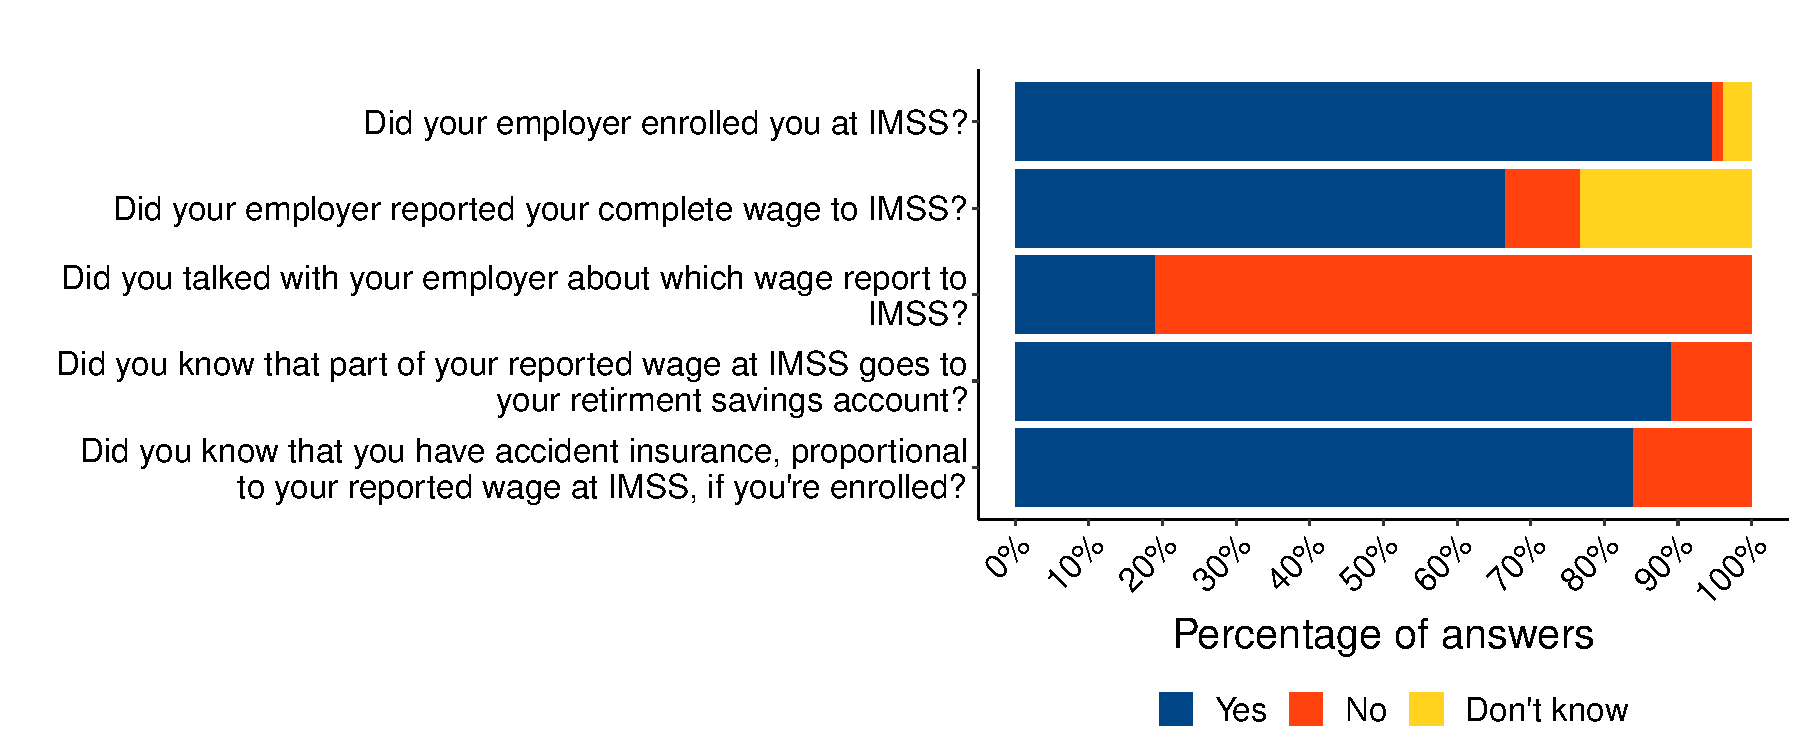
\includegraphics[width=\textwidth]{04_Figures/worker_survey/hist_knowledge_register_survey.pdf}
\end{figure}
\scriptsize{\textit{Notes}: This figure shows answers to questions about IMSS and wage reporting from the worker survey. \textit{Sample:} 233,709 answers from a survey conducted via email to workers enrolled at IMSS during August 2021. Questions 1-2, about the worker's employer, included the option "I don't know". Questions 3-5 ask about the worker's actions or knowledge didn't include the option "I don't know".}

\clearpage

%\subsection{RPCI}

\begin{figure}[H]
    \label{rpci_example}
    \caption{RPCI example}
    \begin{center}
    
    \begin{subfigure}{0.49\textwidth}
    \caption{RPCI within the IMSS Digital app}
    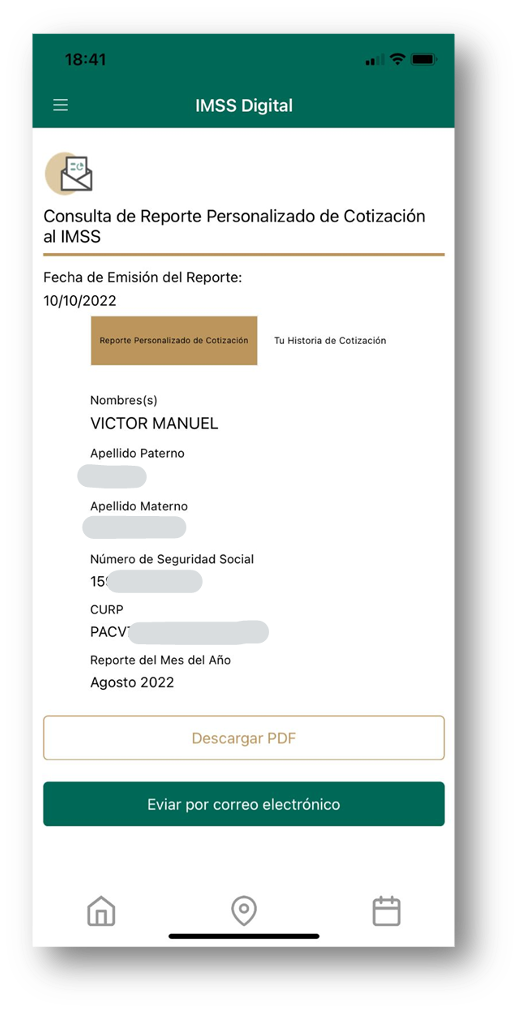
\includegraphics[width=\textwidth]{04_Figures/rpci_app/rpci_2.png}
    \end{subfigure}
    \begin{subfigure}{0.49\textwidth}
    \caption{RPCI PDF file}
    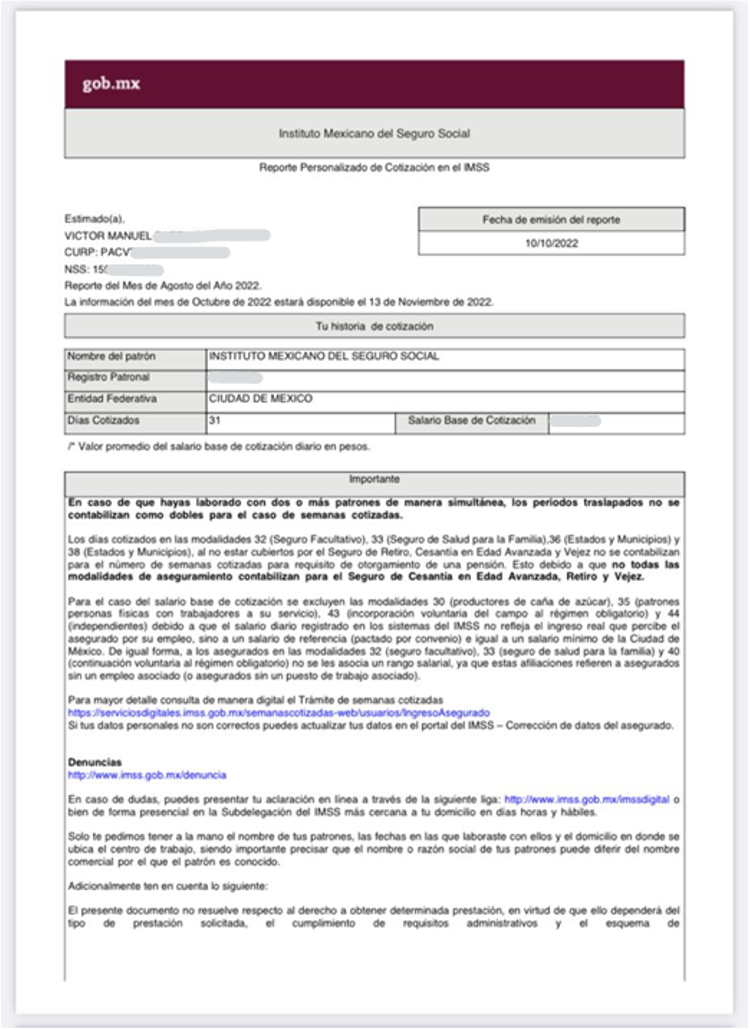
\includegraphics[width=\textwidth]{04_Figures/rpci_app/rpci_3.png}
    \end{subfigure}
    

    \end{center}
\end{figure}
\scriptsize{
\noindent Figure (a) shows the IMSS Digital app, where once the worker is registered for the RPCI, the worker can download their report in PDF or receive it via email. Figure (b) shows an example of the PDF for the RPCI. The report includes the worker job registered information, such as wage and the firm the worker is registered at.
}


 
%\subsection{RPCI registers by month}

\begin{figure}[H]
    \caption{RPCI registers by month}
    \label{hist_download}
    \begin{center}
    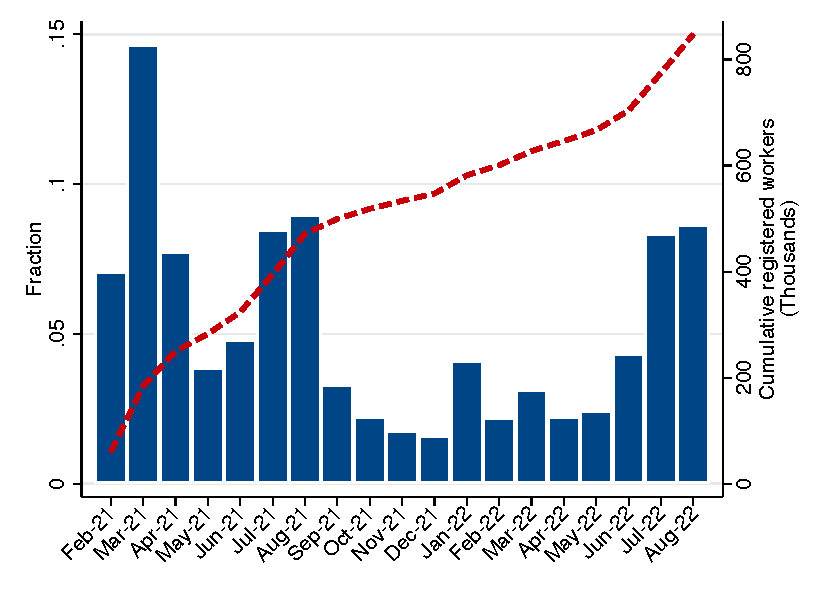
\includegraphics[width=0.65\textwidth]{04_Figures/muestra_1porciento/hist_download_month.pdf}
    \end{center}
\end{figure}
\scriptsize{
\noindent This figure shows the total number of workers registered for the RPCI. The right y-axis measures the fraction of workers who registered for the RPCI during each month from the total workers who registered for the RPCI. The left y-axis measures the cumulative number of workers who registered for the RPCI.
}

\clearpage

%\subsection{Event Studies: RPCI effect on enrollment and wages}

\begin{figure}[H]
    \centering
    \caption{Event studies - RPCI effect on enrollment and wages \label{fig:event_study_rpci}}
    
    \begin{subfigure}{0.49\textwidth}
    \caption{Effect on being enrolled}
    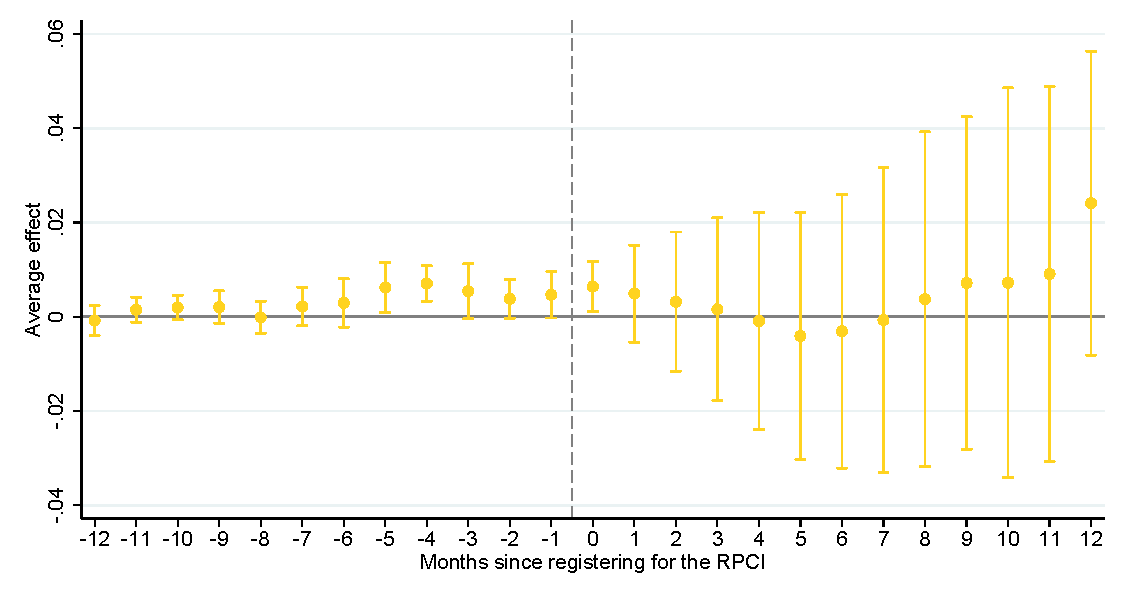
\includegraphics[width=\textwidth]{04_Figures/muestra_10porciento/event_study_alta_dcdh.pdf}
    \end{subfigure}
    
    \begin{subfigure}{0.49\textwidth}
    \caption{Effect on formal wage}
    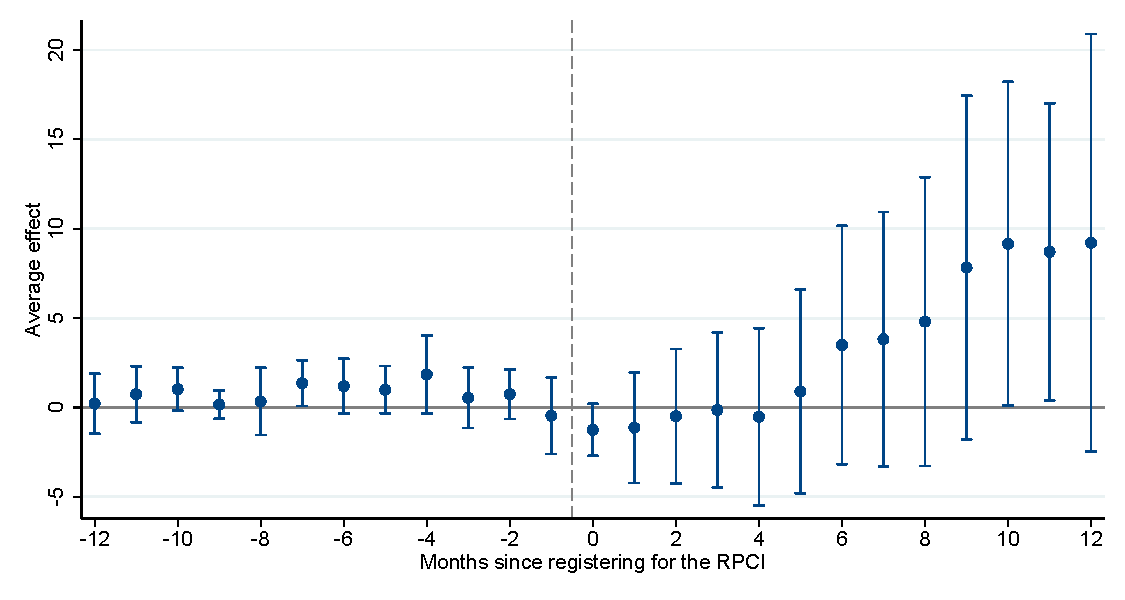
\includegraphics[width=\textwidth]{04_Figures/muestra_10porciento/event_study_sal_formal_dcdh.pdf}
    \end{subfigure}
    \begin{subfigure}{0.49\textwidth}
    \caption{Effect on wage$^\dagger$}
    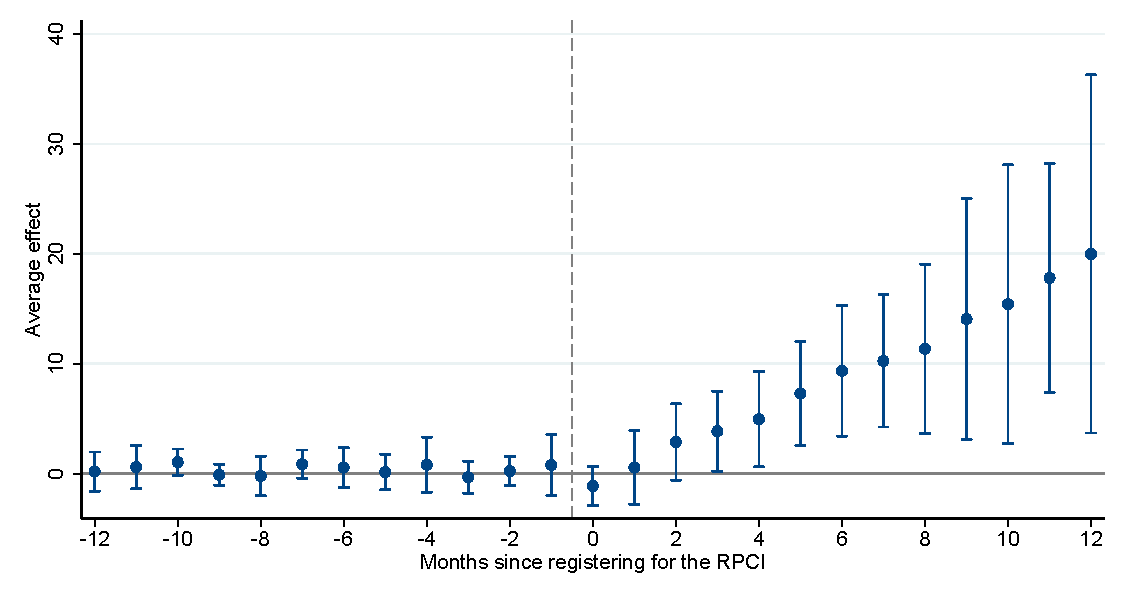
\includegraphics[width=\textwidth]{04_Figures/muestra_10porciento/event_study_sal_cierre_dcdh.pdf}
    \end{subfigure}
    
    %\textit{Do file: event_study_rpci.do}
\end{figure}

\scriptsize{
\noindent \textit{Notes}: This figures shows the event studies for the effect of registering to the RPCI on enrollment and the worker's wage. \textit{Sample:} Panel data for a random sample of the workers enrolled at the Mexican Institute of Social Security (IMSS) during during 2020 and January 2021 (before the RPCI launch). \textit{Enrolled} is a dummy variable where 1 means worker $i$ was enrolled at IMSS during period $t$. $\dagger$ \textit{Formal Wage} and \textit{Wage} are the registered wage for worker $i$ during period $t$, the difference is \textit{Formal Wage} is 0 when the worker isn't enrolled, while \textit{Wage} is missing when the worker isn't enrolled. The event studies follow the estimators proposed by \cite{de2020two}, using the robust dynamic option to account for possible heterogeneous treatment effects across cohorts. Robust standard errors clustered by worker id. This figure is referenced in %\hyperref[subsec:workers]{Section} \ref{subsec:workers}.
}

\clearpage

\begin{comment}
    
%\subsection{Event Studies: RPCI effect on wage changes}

\begin{figure}[H]
    \centering
    \caption{Event studies - RPCI effect on wage changes \label{fig:event_study_wage_changes_rpci}}
    
    \begin{subfigure}{0.49\textwidth}
    \caption{Effect on wage changes}
    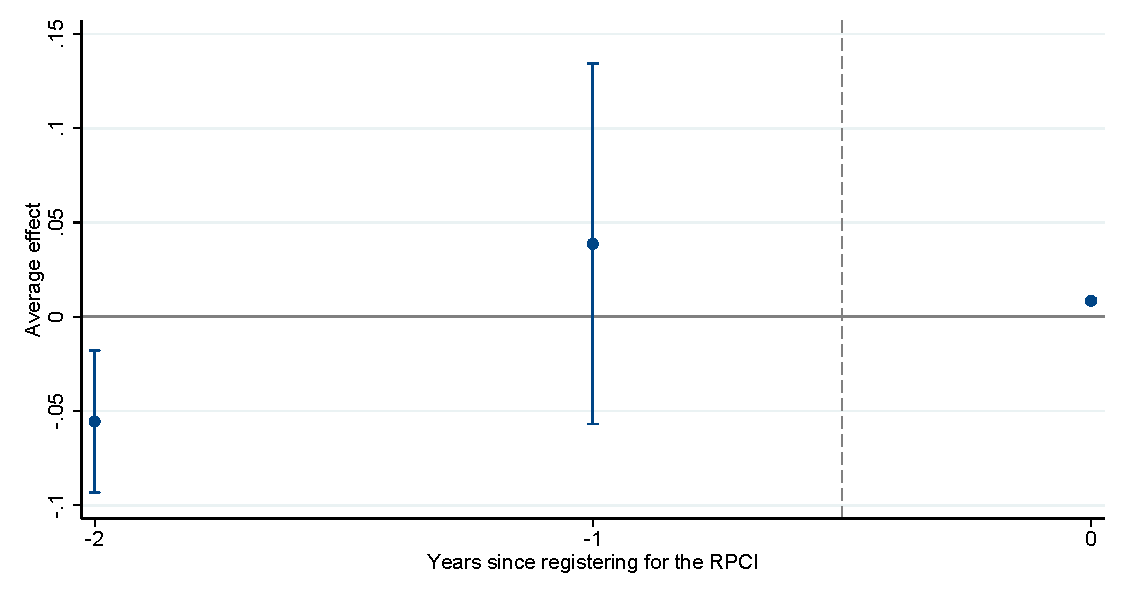
\includegraphics[width=\textwidth]{04_Figures/muestra_10porciento/event_study_sal_diff_yr_dcdh.pdf}
    \end{subfigure}
    
    \begin{subfigure}{0.49\textwidth}
    \caption{Effect on wage raises}
    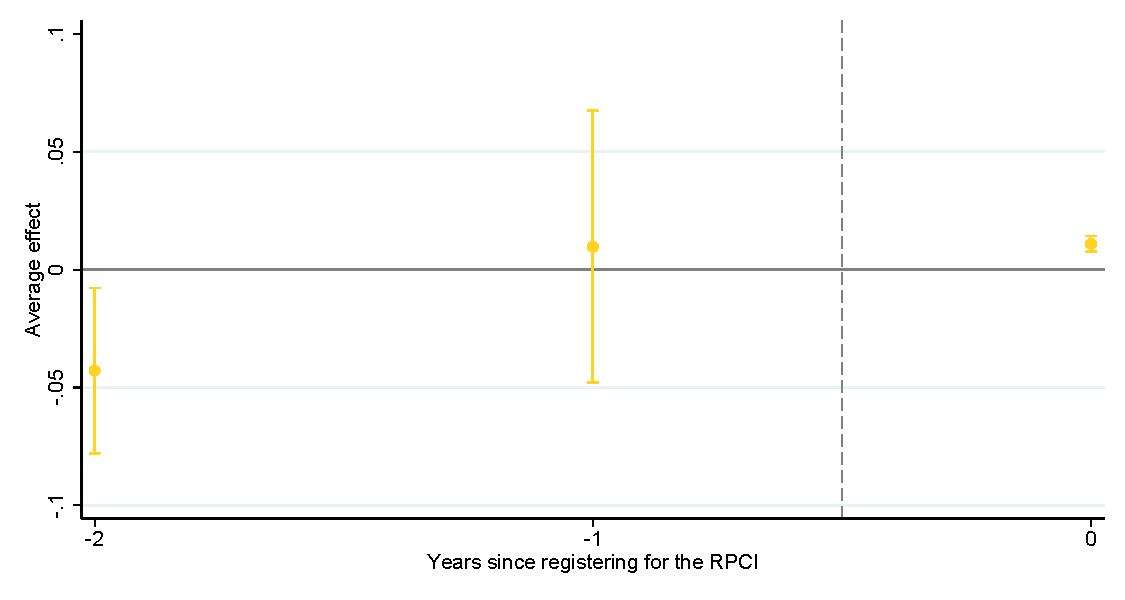
\includegraphics[width=\textwidth]{04_Figures/muestra_10porciento/event_study_sal_mayor_yr_dcdh.pdf}
    \end{subfigure}
    \begin{subfigure}{0.49\textwidth}
    \caption{Effect on wage cuts}
    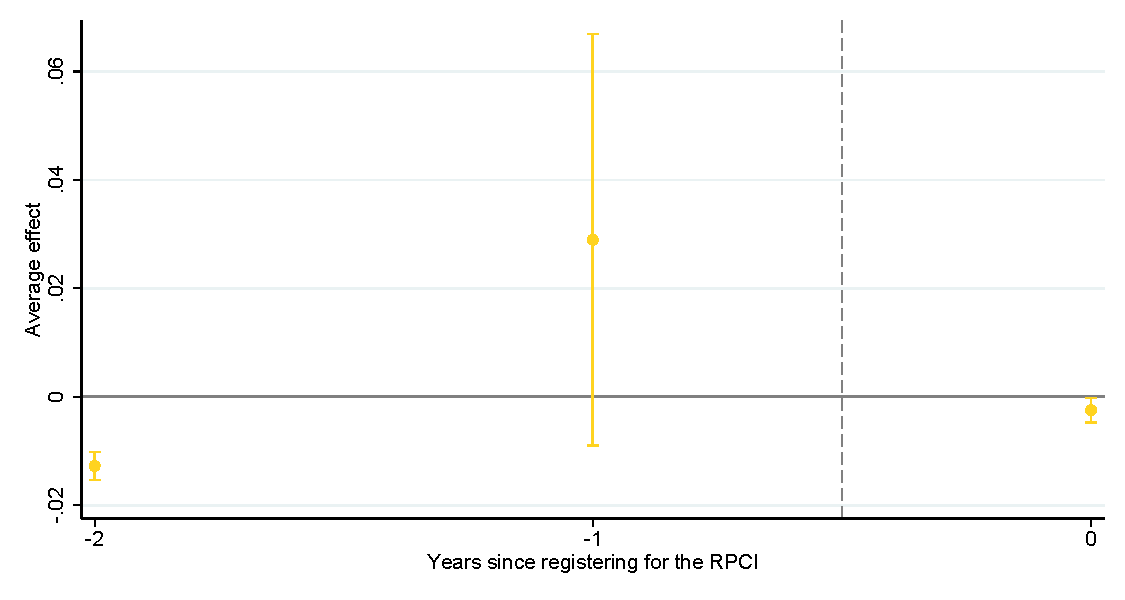
\includegraphics[width=\textwidth]{04_Figures/muestra_10porciento/event_study_sal_menor_yr_dcdh.pdf}
    \end{subfigure}
    
    %\textit{Do file: event_study_rpci.do}
\end{figure}

\scriptsize{
\noindent \textit{Notes}: This figures shows the event studies for the effect of registering to the RPCI on enrollment and the worker's wage. \textit{Sample:} Panel data for a random sample of the workers enrolled at the Mexican Institute of Social Security (IMSS) during during 2020 and January 2021 (before the RPCI launch). \textit{Wage Changes} counts the number of changes in the reported wage at IMSS of worker $i$ during year $t$. \textit{Wage Raises} counts the number of wage changes where the wage increased and \textit{Wage Cuts} counts the number of wage changes where the wage decreased. The event studies follow the estimators proposed by \cite{de2020two}, using the robust dynamic option to account for possible heterogeneous treatment effects across cohorts. Robust standard errors clustered by worker id. This figure is referenced in %\hyperref[subsec:workers]{Section} \ref{subsec:workers}.
}

\end{comment}

\clearpage

%%%%%%%%%%%%%%%%%%%%%%%%%%%%%%%%%%%%%%%%%%%%%%%%%%%%%%

\newpage
%  \documentclass[oneside,11pt]{article}

% 
\usepackage{soul}
\usepackage{natbib}
\usepackage{hyperref}
\usepackage{bookmark}
\usepackage{graphicx}             
\graphicspath{{./Figuras/}}
\usepackage[dvipsnames]{xcolor}
\usepackage{todonotes}
\usepackage{makecell}
\usepackage[margin=1in]{geometry}
\usepackage{float}                
\usepackage{amsmath}
\usepackage{amscd}
\usepackage{amsfonts}
\usepackage{amssymb}
\usepackage{bbm}
\usepackage{booktabs}
\usepackage{nameref}
\usepackage{multirow}
\usepackage[nokeyprefix]{refstyle}
\usepackage{rotating}
\usepackage{threeparttable}
\usepackage{afterpage}
\usepackage{lscape}
\usepackage{enumerate}
\usepackage{caption}
\usepackage{subcaption}
\usepackage{epstopdf}
\usepackage{setspace}
\usepackage{svg}
\usepackage{dsfont}
\usepackage{amsthm}
\usepackage{tocloft}
\usepackage{etoc}
\usepackage{lmodern}
\usepackage{bm}
\usepackage[T1]{fontenc}
\usepackage{tgpagella}

\epstopdfDeclareGraphicsRule{.tiff}{png}{.png}{convert #1 \OutputFile}
\AppendGraphicsExtensions{.tiff}

\epstopdfDeclareGraphicsRule{.tif}{png}{.png}{convert #1 \OutputFile}
\AppendGraphicsExtensions{.tif}

\def\sym#1{\ifmmode^{#1}\else\(^{#1}\)\fi}

\usepackage{tikz}
\usetikzlibrary{shapes.geometric, arrows}
\usetikzlibrary{calc}
\usetikzlibrary{matrix}

\tikzset{ 
    table/.style={
        matrix of nodes,
        row sep=-\pgflinewidth,
        column sep=-\pgflinewidth,
        nodes={
            rectangle,
            draw=black,
            align=center
        },
        minimum height=1.5em,
        text depth=0.5ex,
        text height=2ex,
        nodes in empty cells,
%%
        every even row/.style={
            nodes={fill=gray!20}
        },
        column 1/.style={
            nodes={text width=2em,font=\bfseries}
        },
        row 1/.style={
            nodes={
                fill=black,
                text=white,
                font=\bfseries
            }
        }
    }
}


\usepackage{colortbl}
\usepackage{url}
\urlstyle{rm}
\definecolor{darkblue}{rgb}{0,0,.4}
\hypersetup{colorlinks=true, breaklinks=true, citecolor=Maroon, linkcolor=darkblue, menucolor=darkblue, urlcolor=darkblue}

\newtheorem{theorem}{Theorem}
\newtheorem{claim}[theorem]{Claim}
\newtheorem{prop}[theorem]{Proposition} 
\newtheorem{cor}[theorem]{Corollary} 
\newtheorem{assumption}{Assumption} 
\newtheorem{lem}{Lemma} 

\DeclareRobustCommand{\hlgr}[1]{{\sethlcolor{green}\hl{#1}}}


\usepackage{comment}
%para esconder columnas en tablas (enrique)
\usepackage{array}
\newcolumntype{H}{>{\setbox0=\hbox\bgroup}c<{\egroup}@{}}
\linespread{1.25}

\newcommand{\wh}{\widehat}
\usepackage{anyfontsize}

\usepackage[linesnumbered,vlined,ruled,commentsnumbered]{algorithm2e}

\DontPrintSemicolon
\newcommand{\To}{\mbox{\upshape\bfseries to}}
\newcommand{\E}{\mathbb{E}}

\DeclareCaptionFormat{cont}{#1 (cont.)#2#3\par}
% %%% HELPER CODE FOR DEALING WITH EXTERNAL REFERENCES
% \usepackage{xr}
% \makeatletter
% \newcommand*{\addFileDependency}[1]{
%   \typeout{(#1)}
%   \@addtofilelist{#1}
%   \IfFileExists{#1}{}{\typeout{No file #1.}}
% }
% \makeatother


% \newcommand*{\myexternaldocument}[1]{
%     \externaldocument{#1}
%     \addFileDependency{#1.tex}
%     \addFileDependency{#1.aux}
% }

% %\myexternaldocument{OA}

% %%%%%%%%%%%%%%%%%%%%%%%%%%%%%%%% DOCUMENT
% \begin{document}

%%%%%%%%%%%%%%%%%%%%%%%%%%%%%%%%%%%%%%%%%%%%%%%

% APPENDIX 
\setcounter{table}{0}
\setcounter{figure}{0}
\setcounter{section}{0}
\pagenumbering{gobble}


\begin{center}
	\LARGE IMSS RPCI \\[0.5em]
	\Large{Appendix $-$ For Online Publication} \\[1em]
	\large \author{Eduardo Alcaraz \and Gabriela López \and Luis Martínez \and Marco Medina \and Enrique Seira}
\end{center}

\appendix
\pagenumbering{arabic}
\renewcommand\thefigure{OA-\arabic{figure}}
\renewcommand\thetable{OA-\arabic{table}}
\renewcommand*{\thepage}{OA - \arabic{page}}
\renewcommand\thesection{Appendix \Alph{section}.}
\renewcommand\thesubsection{\Alph{section}.\arabic{subsection}}

%\renewcommand{\cftparskip}{0em} % NOT NEEDED
\renewcommand\cftsecdotsep{\cftdotsep}
\renewcommand\cftsubsecdotsep{\cftnodots}
\renewcommand{\cftsecnumwidth}{6em}
 \renewcommand{\cftpnumalign}{r}
%\renewcommand{\cftsecleader}{\normalfont\cftdotfill{\cftsecdotsep}}


\renewcommand{\cftsecleader}{\cftdotfill{\cftsecdotsep}\hspace{1.8em}}
%\renewcommand{\cftsecpagefont}{20em}
%\renewcommand{\cftfignumwidth}{6em}
%\renewcommand{\cfttabnumwidth}{3.3em}

%\tableofcontents
\etocdepthtag.toc{mtappendix}
\etocsettagdepth{mtchapter}{none}
\etocsettagdepth{mtappendix}{subsection}

\setstretch{0.9}
%\renewcommand\contentsname{} % the empty name

\begingroup
\let\clearpage\relax
%\vspace{-1.5em} % the removed space. Set as appropriate
\tableofcontents
\endgroup

\clearpage

\section{ RPCI}
\vspace{.2in}

\begin{figure}[H]
    \caption{RPCI flyers}
    \label{rpci_flyers}
    \begin{center}
    
    \begin{subfigure}{0.49\textwidth}
    \caption{RPCI flyer titled "Does my employer has me registered at IMSS?"}
    
\includegraphics[width=\textwidth]{04_Figures/rpci_app/rpci_flyer_3.jpeg}
    \end{subfigure}
    \begin{subfigure}{0.49\textwidth}
    \caption{RPCI flyer titled "Digital services for a healthy environment"}
    
\includegraphics[width=\textwidth]{04_Figures/rpci_app/rpci_flyer_2.jpeg}
    \end{subfigure}

    \end{center}
\end{figure}
\scriptsize{
\noindent Flyers circulated by the Mexican Institute of Social Security (IMSS) for the RPCI. Both flyers explain how you can track and access your job register information, such as wage and firm you are registered at, if you register for the RPCI.
}

\clearpage

\begin{figure}[H]
    \caption{Registering for the RPCI}
    \label{rpci_register}
    \begin{center}
    
    \begin{subfigure}{0.9\textwidth}
    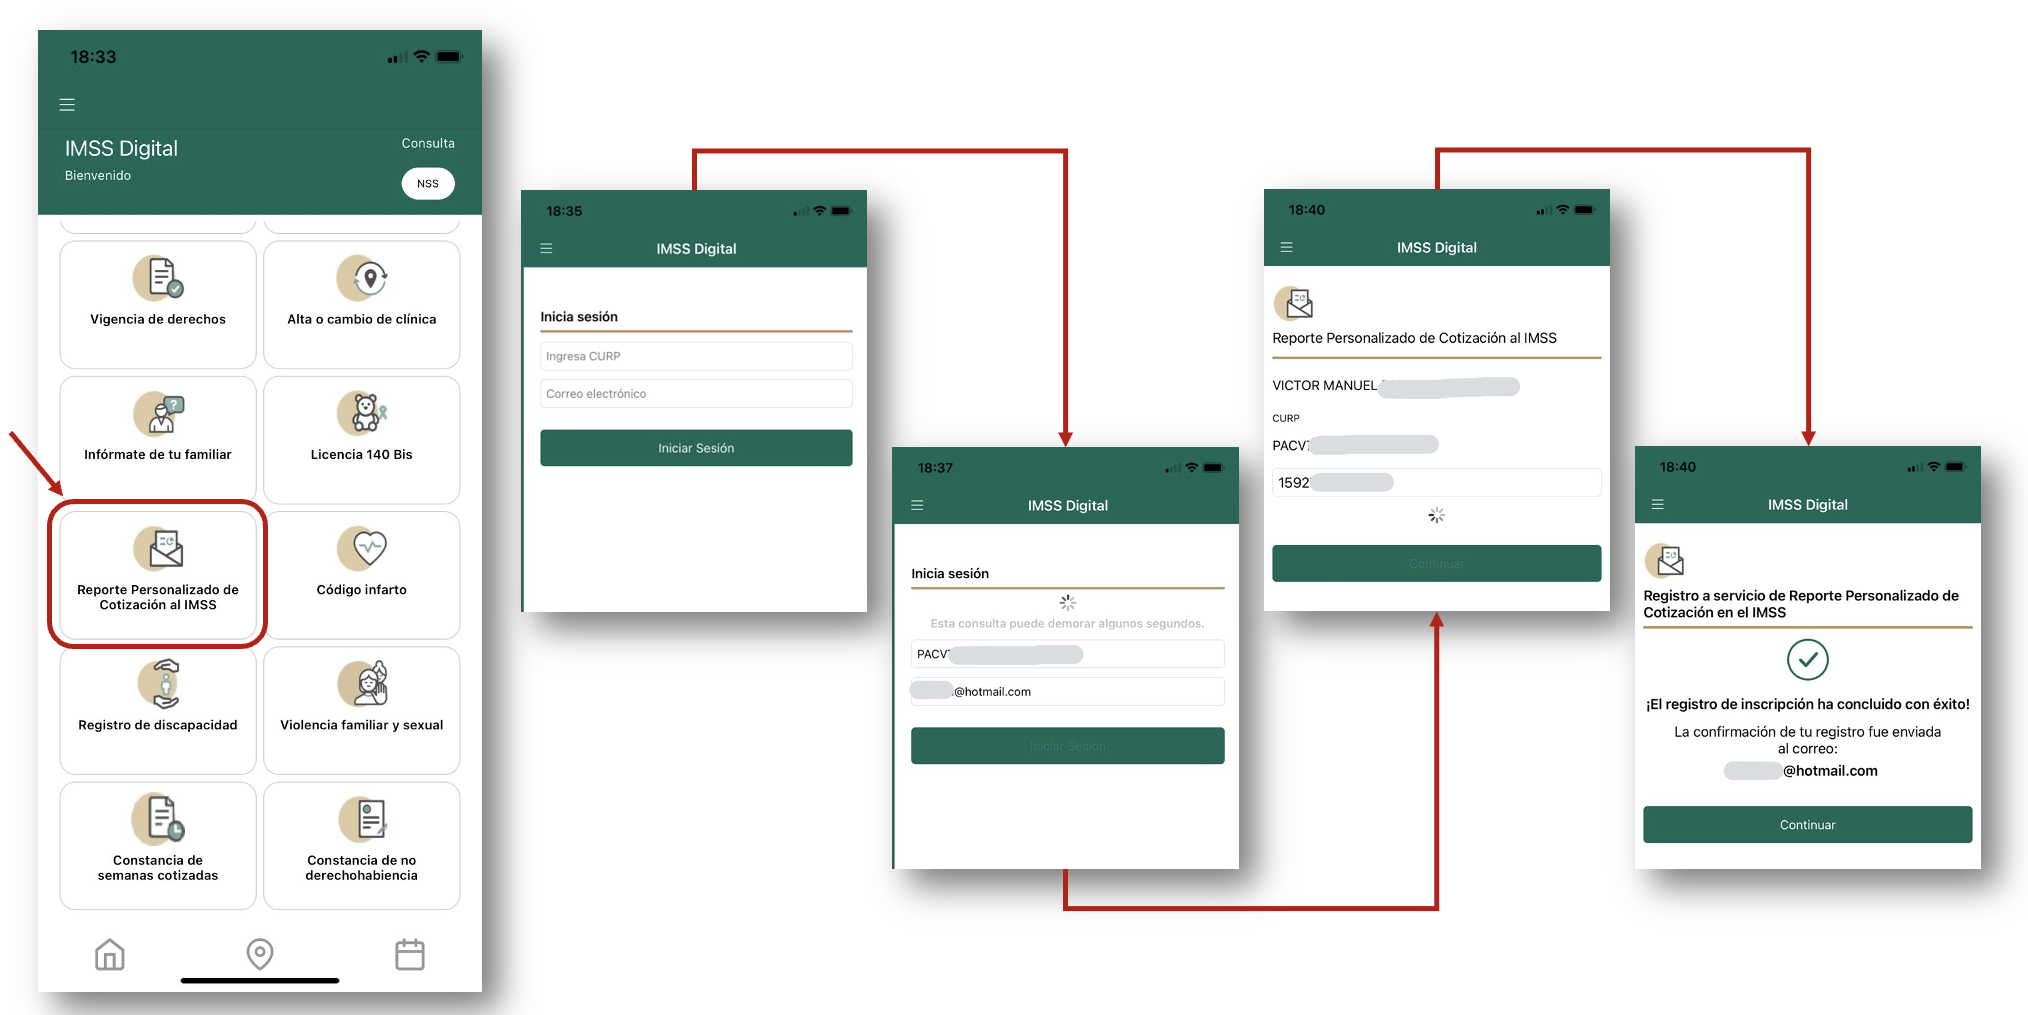
\includegraphics[width=\textwidth]{04_Figures/rpci_app/rpci_register.png}
    \end{subfigure}

    \end{center}
\end{figure}
\scriptsize{
\noindent Diagram shows how to register for the RPCI within the IMSS Digital app. The worker registers only once to access the RPCI, using his Unique Population Registry Key (CURP) and email address.
}

\clearpage

\begin{figure}[H]
    \caption{RPCI example}
    \label{rpci_example}
    \begin{center}
    
    \begin{subfigure}{0.49\textwidth}
    \caption{RPCI within the IMSS Digital app}
    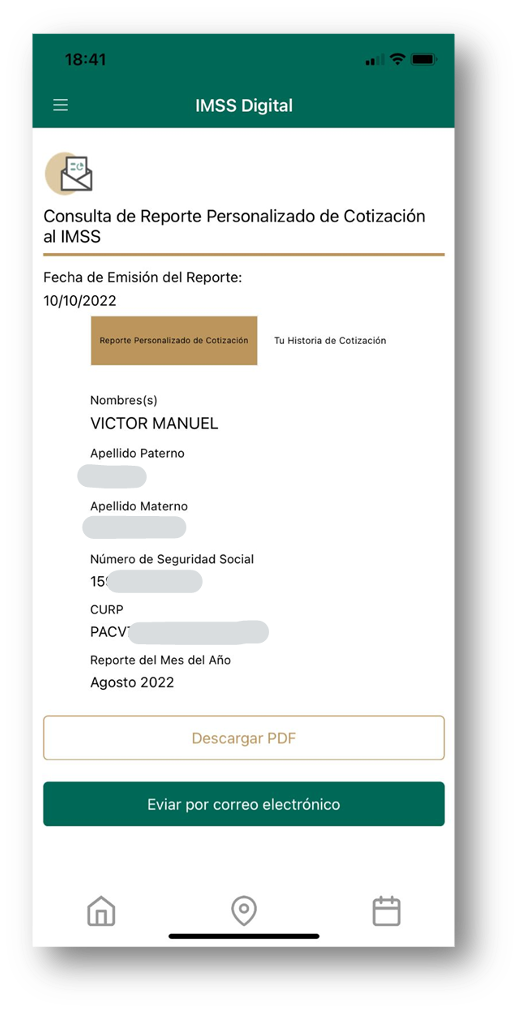
\includegraphics[width=\textwidth]{04_Figures/rpci_app/rpci_2.png}
    \end{subfigure}
    \begin{subfigure}{0.49\textwidth}
    \caption{RPCI PDF file}
    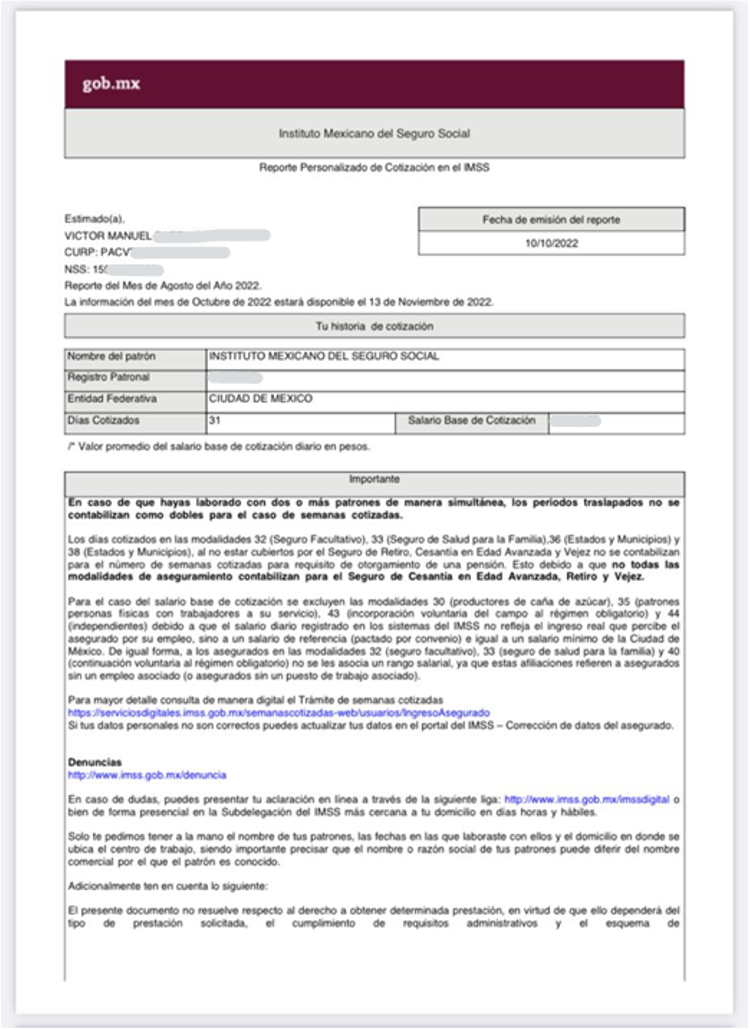
\includegraphics[width=\textwidth]{04_Figures/rpci_app/rpci_3.png}
    \end{subfigure}
    

    \end{center}
\end{figure}
\scriptsize{
\noindent Figure (a) shows the IMSS Digital app, where once the worker is registered for the RPCI, the worker can download their report in PDF or receive it via email. Figure (b) shows an example of the PDF for the RPCI. The report includes the worker job registered information, such as wage and the firm the worker is registered at.
}

%\clearpage

%\bibliographystyle{authordate1}
%\bibliographystyle{amsalpha}
%\bibliographystyle{AER}

%\bibliography{References}




% \end{document}

\end{document}

